\documentclass[10pt]{article}

% small margins
\usepackage[margin=1in]{geometry}

% no large spaces in lists
\usepackage{enumitem}
\setlist{nolistsep}

\title{\vspace{-4em}6.S078 Update}
\author{Troy Astorino \and Turner Bohlen \and Craig Cheney \and Gus Downs}
\date{March 5, 2013}

\usepackage{pdfpages}

\begin{document}
\maketitle
\vspace{-4em}

\section{Plan Progress}
As a quick reminder, we are working on building a low-cost, high precision 3D
scanner. Beyond low cost and high accuracy, we have design goals of a modular
design that can be expanded, and compact design that can fit on a desk. We see
our target users as general consumers and budget-constrained professionals, e.g.
small manufacturing plants, research labs, designers, artists, etc.

We have continued with our technology and market research from last week, and are more
confident in our market assumptions. We are securing funding for prototype
development, and working on software in parallel with the hardware development
(developing software with larger camera/projector systems while our hardware is
being developed).

\section{Prototype Progress}
We made a very crude initial CAD model, and have started writing general
software that works with large scale projector and camera systems, but will also
work with our sensors.  We're working so that the hardware and software
development can move in parallel.

We've established a few different imaging and projection techniques we're going
to try, so we can see which will be most effective for us to achieve our design
goals. The techniques we are trying are:
\begin{itemize}
\item Projection Ideas
\begin{itemize}
\item Small grating in front of an LED. The shadow created by the grating on the
  object will create the lines necessary for structured light scanning.  We will
  investigate having multiple static LEDs projecting from different angles, and
  having a single LED that casts a shifting shadow because the grating moves in
  front of it.
\item Overlapping color filters. Have multiple filter sheets (red, green, blue,
  etc.) with holes cut in them. Have the holes overlap irregularly, so a
  multi-colored grid is projected on the object to be scanned
\item Manufacture our own projector. This may be necessary in order to have a
  projection system with a very short focal distance, and may help us lower
  costs
\item Use a pico-projector. An off the shelf pico-projector like those being
  integrated in cell-phones might be the most cost effective solution.  The
  usability of this option depends on the focal range of the projector. The
  object could be spun in front of this projector, or fiber-optics could be used
  to allow projection from different directions with the same projector
\end{itemize}

\item Imaging ideas
\begin{itemize}
\item Array of cheap off-the-shelf CMOS cameras. Could be the ones used cell
  phones.  May have issues with a small focal range, and being in focus for very
  near objects.
\item Manufacture own pinhole camera.  Can use the same CMOS array as those in
  cell phone cameras, but without the lens.  Gives us a larger focal range, but
  may have issues with not enough light.
\end{itemize}
\end{itemize}

\section{Baffling Variables}
The most baffling variable is how well we are going to be able to execute on our
design goals: high precision and low cost. We will not really be able to answer
the high precision question until we have a working prototype. To help answer
the low cost question, we are meeting with a consumer optics consultant to
discuss different techniques we are considering.

These questions will be clarified after we have build working prototype.

\section{Seven Day Plan}
\begin{itemize}
\item Secure funding
\item Order parts for initial prototyping
\item Have a CAD model of a scanned object using a regular projector and a
  webcam
\item Have a rough overall software model for how different components will
  interact, and for how we'll support multiple sources for depth data.
\end{itemize}

\section{People to Meet}
Professor Gifford has kindly introduced us to Dr. Stephen Fantone, who does some
consulting work for consumer products requiring optical solutions.  We are
meeting with him next Tuesday.

We have been trying to get in contact Wojciech Matusik, since his lab does work
in 3D scanning, but we haven't been able to get in contact with him over email.
We may start waiting outside his office (a meeting isn't critical, so we haven't
done this yet).

\section{Desired Resources}
We're in the midst of going through a funding process with Professor Gifford,
and so are in the process of meeting all of our desires for resources. The
slides we sent out for review by the course's VC partners are included in the email.

\begin{appendix}
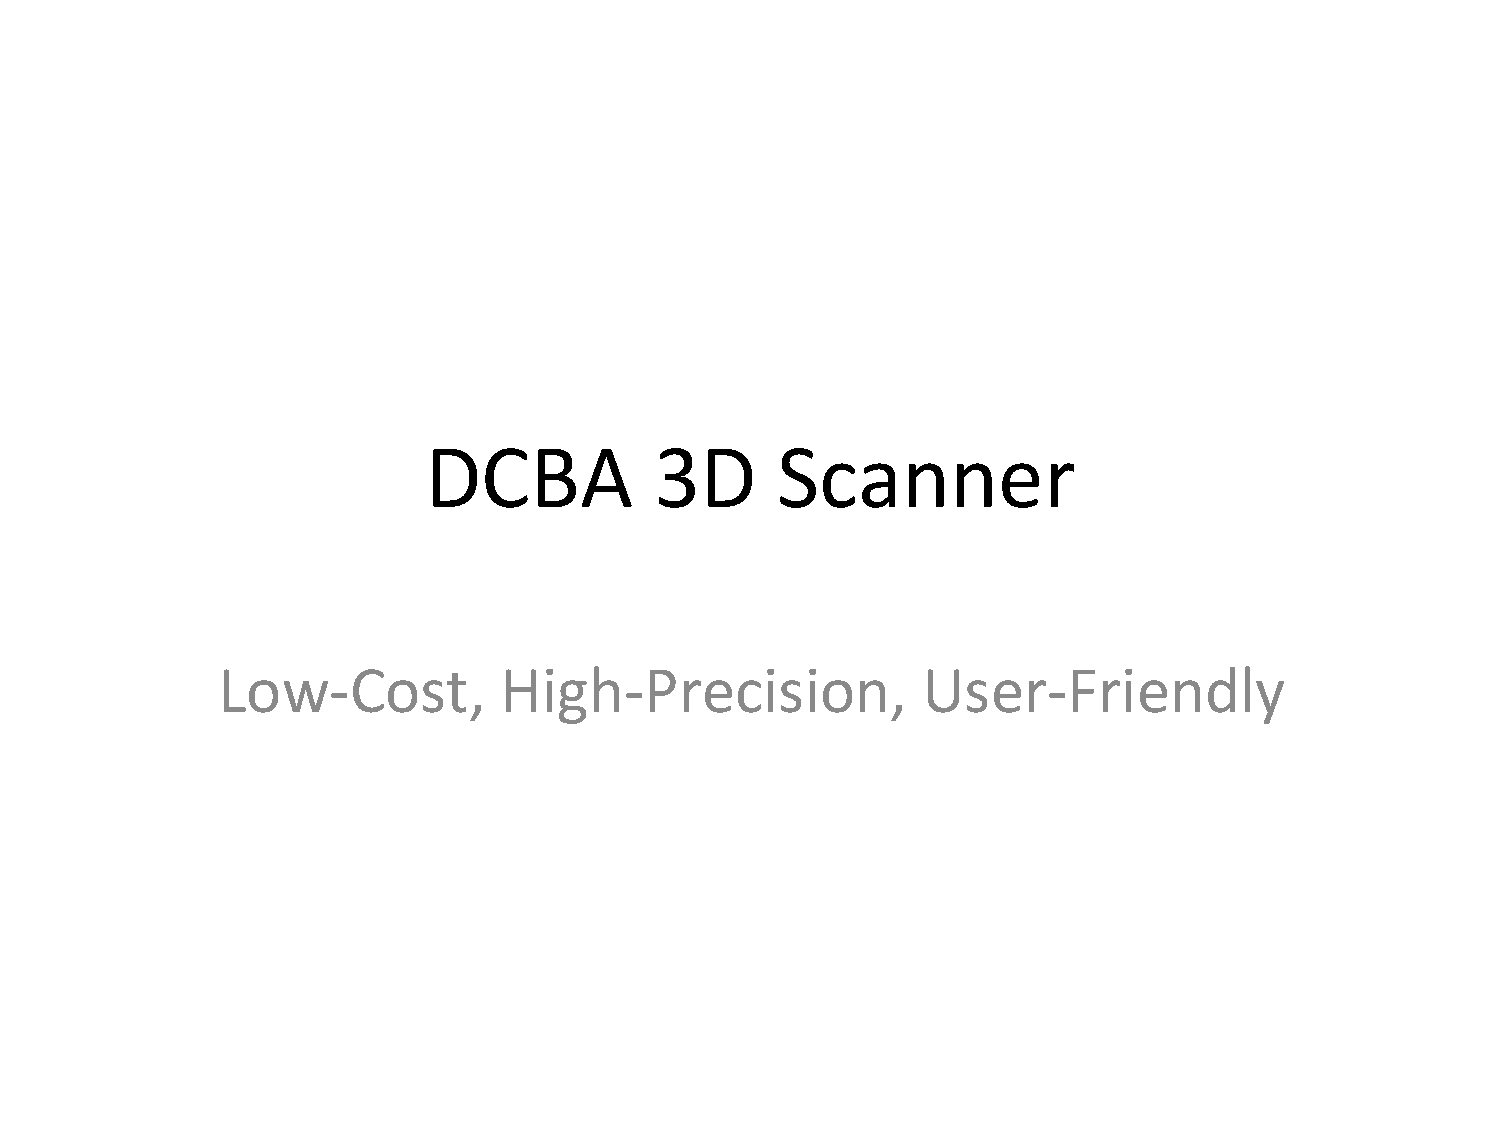
\includepdf[pages={-}]{../../presentations/10-slide-pitch/initial-10-slide-pitch.pdf}
\end{appendix}
\end{document}